\subsection{Adjunction}

Let E be an extension of a field K. Given a family \(\mathbf{x} = (x_{i})_{i \in I}\) of elements of E, we denote by \(\mathrm{K}(x_{i})_{i \in I}\) (or \(\mathrm{K}(\mathbf{x})\) or also \(\mathrm{K}(x_{1}, \ldots, x_{n})\) when I is the interval {[}1, n{]} of N) the least subextension of E containing the members of the family \((x_{i})\) ; we say that \(\mathrm{K}(x_{i})_{i\in I}\) is obtained by adjunction to K of the elements of the family \((x_{i})_{i\in I}\) and that the family \((x_{i})_{i\in I}\) (or the set of its elements) is a generating family of \(\mathrm{K}(x_{i})_{i\in I}\) with respect to K (or over K). The field \(\mathrm{K}(x_{i})_{i\in I}\) depends only on the set A of elements of the family \((x_{i})_{i\in I}\) ; we also denote it by \(\mathrm{K}(\mathrm{A})\) . In particular we have \(\mathrm{K}(\mathrm{E})=\mathrm{E}\) and \(\mathrm{K}(\emptyset)=\mathrm{K} \cdot 1\) . All that has been said applies in particular when E is a field containing K as subfield.

\pandocbounded{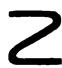
\includegraphics[keepaspectratio]{images/part001_724f36f3.jpg}}

It should be observed that A is not in general a generating set of the algebra \(\mathbf{K}(\mathbf{A})\) , in other words that \(\mathbf{K}(\mathbf{A}) \neq \mathbf{K}[\mathbf{A}]\) . * Nevertheless we shall see that \(\mathbf{K}(\mathbf{A}) = \mathbf{K}[\mathbf{A}]\) when \(\mathbf{K}(\mathbf{A})\) is an algebraic extension of \(\mathbf{K}\) (V, p.~18, Cor. 1) . *

PROPOSITION 2. --- If M and N are any two subsets of an extension of a field K, then \(\mathbf{K}(\mathbf{M} \cup \mathbf{N}) = \mathbf{K}(\mathbf{M})(\mathbf{N}) = \mathbf{K}(\mathbf{N})(\mathbf{M})\) .

For \(\mathbf{K}(\mathbf{M} \cup \mathbf{N})\) contains \(\mathbf{K}(\mathbf{M})\) and \(\mathbf{N}\) and hence \(\mathbf{K}(\mathbf{M})(\mathbf{N})\) ; since \(\mathbf{K}(\mathbf{M})(\mathbf{N})\) is a field containing \(\mathbf{K} \cup \mathbf{M} \cup \mathbf{N}\) , it contains \(\mathbf{K}(\mathbf{M} \cup \mathbf{N})\) , whence the proposition.

We shall sometimes write \(\mathbf{K}(\mathbf{M},\mathbf{N})\) instead of \(\mathbf{K}(\mathbf{M}\cup \mathbf{N})\) .

Remark. --- Let P be the prime subfield of a field E (V, p.~2) ; for every subset A of E, P(A) is the least subfield of E containing A. In particular if K is a subfield of E, we have P(K ∪ A) = K(A). If K and K' are two subfields of E, we thus have P(K ∪ K') = K(K') = K'(K) ; this field is the least subfield of E containing K or K', or also the upper bound of K and K' in the set of subfields of E, ordered by inclusion ; we sometimes say that this field is the field generated by K and K' in E.

PROPOSITION 3. --- Let F be a set of subfields of a field E, directed with respect to the relation ⊂. The union L of the fields of F is a field.

For if \(x\) and \(y\) are two elements of \(L\) , there exist two fields \(R, S\) of \(\mathcal{F}\) such that \(x \in R\) , \(y \in S\) ; let \(T\) be a field of \(\mathcal{F}\) containing \(R\) and \(S\) ; then \(x \in T\) , \(y \in T\) , hence \(x + y\) , \(xy\) and \(x^{-1}\) (if \(x \neq 0\) ) belong to \(T\) , hence to \(L\) .

COROLLARY. --- Let E be an extension of a field K and A ⊂ E. The field K(A) is the union of the fields K(F) where F ranges over the set of all finite subsets of A.

For the set of fields \(\mathbf{K}(\mathbf{F})\) is directed by the relation \(\subset\) , because \(F \subset F'\) implies \(\mathbf{K}(\mathbf{F}) \subset \mathbf{K}(\mathbf{F}')\) . The union L of these fields is thus a field containing \(K \cup A\) and contained in \(\mathbf{K}(\mathbf{A})\) , and hence identical with \(\mathbf{K}(\mathbf{A})\) .

DEFINITION 2. --- An extension E of a field K is said to be finitely generated if it has a finite generating family. It is called monogenous if there exists x in E such that \(E = K(x)\) .

\pandocbounded{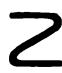
\includegraphics[keepaspectratio]{images/part001_c96515a7.jpg}}

The Cor. of Prop. 3 shows that every extension E of a field K is a directed union of finitely generated extensions contained in E. It is clear that every extension E of K of finite degree is also finitely generated because a basis of E (considered as vector space over K) is also a generating family of E over K; we shall see later that the converse does not hold.

